\documentclass[border=10pt]{standalone}
\usepackage{tikz}

\begin{document}

% We use a minipage-like structure or just side-by-side tikz pictures
% This single document contains both diagrams for easy comparison.

\begin{tabular}{cc}


  % --- Left Diagram: NOT (A AND B) ---
  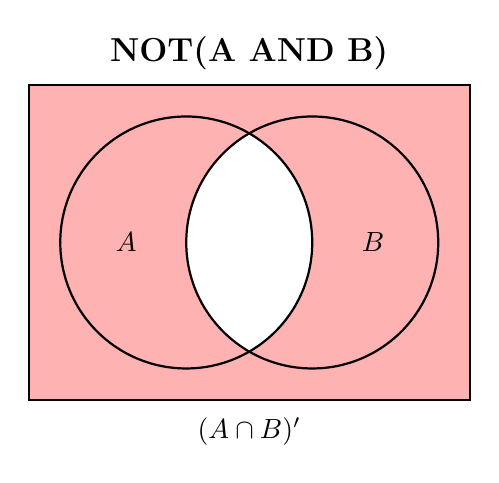
\begin{tikzpicture}[scale=0.8]
    % Define coordinates
    \coordinate (A) at (-1, 0);
    \coordinate (B) at (1, 0);
    \def\radius{2}
    \def\rectW{7}
    \def\rectH{5}

    % Fill Universe (Red)
    \fill[red!30] (-\rectW/2, -\rectH/2) rectangle (\rectW/2, \rectH/2);

    % Clip the intersection region to "unfill" it
    \begin{scope}
      \clip (A) circle (\radius);
      \clip (B) circle (\radius);
      \fill[white] (-\rectW/2, -\rectH/2) rectangle (\rectW/2, \rectH/2);
    \end{scope}

    % Outlines
    \draw[thick] (A) circle (\radius) node[left=0.5cm] {$A$};
    \draw[thick] (B) circle (\radius) node[right=0.5cm] {$B$};
    \draw[thick] (-\rectW/2, -\rectH/2) rectangle (\rectW/2, \rectH/2);

    % Label
    \node at (0, \rectH/2 + 0.5) {\large \textbf{NOT(A AND B)}};
    \node at (0, -\rectH/2 - 0.5) {$(A \cap B)'$};
  \end{tikzpicture}
  
  &  % Separator column
  
  % --- Right Diagram: NOT(A) OR NOT(B) ---
  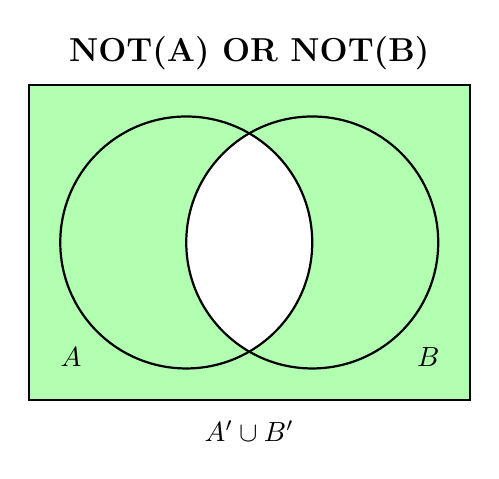
\begin{tikzpicture}[scale=0.8]
    % Define coordinates
    \coordinate (A) at (-1, 0);
    \coordinate (B) at (1, 0);
    \def\radius{2}
    \def\rectW{7}
    \def\rectH{5}

    % Logic: The union of "Outside A" and "Outside B" 
    % results in everything EXCEPT the intersection.
    % Visually, this is identical to the left diagram.
    
    % Fill Universe (Green)
    \fill[green!30] (-\rectW/2, -\rectH/2) rectangle (\rectW/2, \rectH/2);

    % Unfill the intersection
    \begin{scope}
      \clip (A) circle (\radius);
      \clip (B) circle (\radius);
      \fill[white] (-\rectW/2, -\rectH/2) rectangle (\rectW/2, \rectH/2);
    \end{scope}

    % Outlines
    \draw[thick] (A) circle (\radius) node[below left=1.2cm] {$A$};
    \draw[thick] (B) circle (\radius) node[below right=1.2cm] {$B$};
    \draw[thick] (-\rectW/2, -\rectH/2) rectangle (\rectW/2, \rectH/2);

    % Label
    \node at (0, \rectH/2 + 0.5) {\large \textbf{NOT(A) OR NOT(B)}};
    \node at (0, -\rectH/2 - 0.5) {$A' \cup B'$};
  \end{tikzpicture}

\end{tabular}

\end{document}